\documentclass[12pt,border=0pt]{standalone}

\usepackage[utf8]{inputenc} 
\usepackage{amssymb,amsmath}
\usepackage{tikz}



\thispagestyle{empty}

\begin{document}

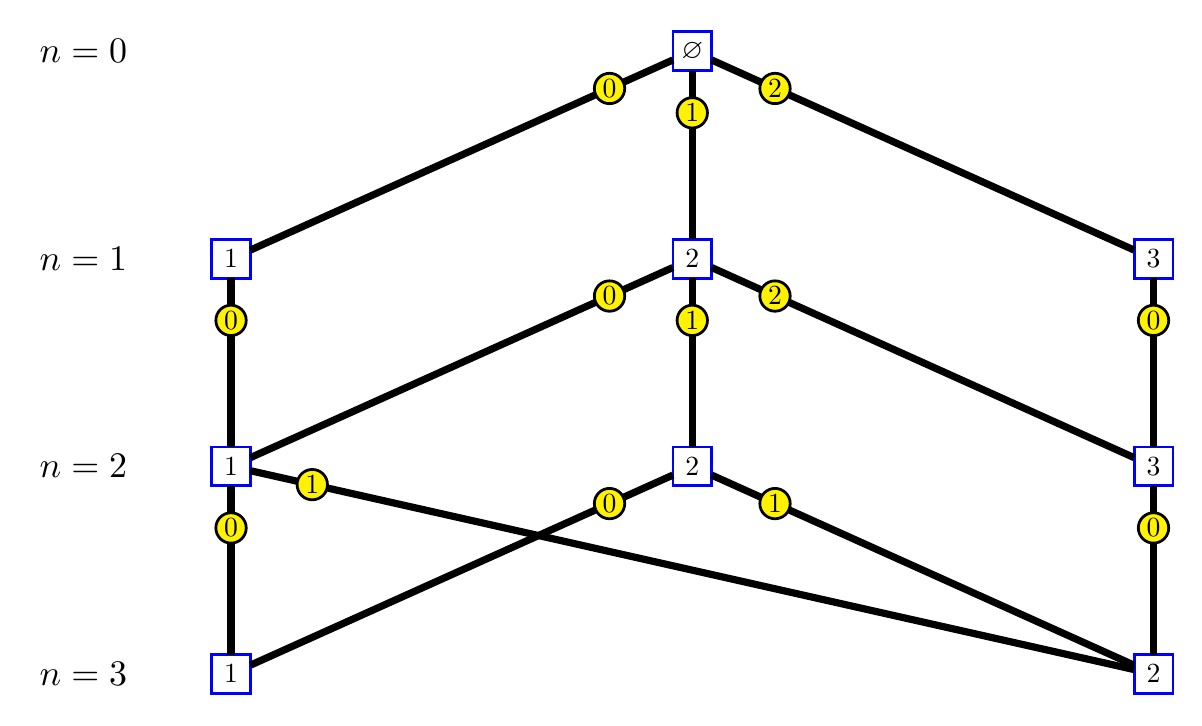
\begin{tikzpicture}[x=10pt,y=6pt]
  \centering
  \tikzset{VertexStyle/.style = {
    shape         = rectangle,
    draw          = blue, 
    fill          = white, 
  	line width    = 1pt, 
    text          = black,
    inner sep     = 1pt,
    outer sep     = 0pt,
    minimum size  = 14 pt,
    scale         = 1
    }
  }
  \tikzset{EdgeStyle/.style = {
    draw            = black, 
    thick,
    double          = black,
    double distance = 1pt
    }
  }
  \tikzset{EdgeLabelStyle/.style = {
    draw          = black,
  	shape         = circle, 
  	line width    = 1pt, 
  	minimum size  = 10pt, 
    inner sep     = 1pt,
    outer sep     = 0pt,
    fill          = yellow,
    text          = black,
    scale         = 1,
    pos = 0.25
    }
  }

	\node[VertexStyle](A1) at (25, 43.75) {$\varnothing$};
	\node[VertexStyle](B1) at (8.33333333333333, 31.25) {$1$};
	\node[VertexStyle](B2) at (25, 31.25) {$2$};
	\node[VertexStyle](B3) at (41.6666666666667, 31.25) {$3$};
	\node[VertexStyle](C1) at (8.33333333333333, 18.75) {$1$};
	\node[VertexStyle](C2) at (25, 18.75) {$2$};
	\node[VertexStyle](C3) at (41.6666666666667, 18.75) {$3$};
	\node[VertexStyle](D1) at (8.33333333333333, 6.25) {$1$};
	\node[VertexStyle](D2) at (41.6666666666667, 6.25) {$2$};
	\draw[EdgeStyle](A1) to node[EdgeLabelStyle, pos=0.15]{$0$} (B1);
	\draw[EdgeStyle](A1) to node[EdgeLabelStyle]{$1$} (B2);
	\draw[EdgeStyle](A1) to node[EdgeLabelStyle, pos=0.15]{$2$} (B3);
	\draw[EdgeStyle](B1) to node[EdgeLabelStyle]{$0$} (C1);
	\draw[EdgeStyle](B2) to node[EdgeLabelStyle, pos=0.15]{$0$} (C1);
	\draw[EdgeStyle](B2) to node[EdgeLabelStyle]{$1$} (C2);
	\draw[EdgeStyle](B2) to node[EdgeLabelStyle, pos=0.15]{$2$} (C3);
	\draw[EdgeStyle](B3) to node[EdgeLabelStyle]{$0$} (C3);
	\draw[EdgeStyle](C1) to node[EdgeLabelStyle]{$0$} (D1);
	\draw[EdgeStyle](C1) to node[EdgeLabelStyle, pos=0.07]{$1$} (D2);
	\draw[EdgeStyle](C2) to node[EdgeLabelStyle, pos=0.15]{$0$} (D1);
	\draw[EdgeStyle](C2) to node[EdgeLabelStyle, pos=0.15]{$1$} (D2);
	\draw[EdgeStyle](C3) to node[EdgeLabelStyle]{$0$} (D2);


	\node[scale=1.3](n3) at (3, 6.25) {$n=3$};
	\node[scale=1.3](n2) at (3, 18.75) {$n=2$};
	\node[scale=1.3](n1) at (3, 31.25) {$n=1$};
	\node[scale=1.3](n0) at (3, 43.75) {$n=0$};	
	
  \end{tikzpicture}

\end{document}
